\section{Разработка backend части приложения}

\subsection{Постановка задачи}
В существующих backend технологиях наблюдается большое разнообразие, и каждый из языков или фреймворков предлагает свои преимущества. Так, например, Discord использует Elixir в задачах, связанных с многопоточностью\cite{discord-elixir} и Rust в местах, где необходима максимальная производительность\cite{discord-rust}. Сочетание нескольких языков для наиболее эффективного решения задачи --- не редкость. В своей работе мы также можем не привязываться к технологиям, используемым в фронтенде приложения, тем не менее, мы остановим свой выбор на TypeScript --- единый язык позволит облегчить поддержку сервиса, кроме того JavaScript/Type\-Script обладает развитой экосистемой библиотек, пакетов, инструментов и широкой поддержкой по платформам.

В данном разделе мы ставим цель реализовать все сервисы, которые использует фронтенд --- мобильное приложение. Так возникает задача разработки следующих компонентов:
\begin{itemize}
	\item Регистрация и аутентификация пользователей.
	\item Хранение истории изученных слов, прохождения тестов, настроек и прочих данных, а также синхронизация этой информации между устройствами.
	\item Сервис проверки и анализа произношения.
	\item Сервис генерации текста заданной направленности.
	\item Сервис синтеза речи.
	\item Сервис классификации текста по темам.
	\item Контроль доступа пользователей к контенту.
\end{itemize}

Далее в этом разделе мы рассмотрим реализацию поставленных задач и интеграцию этих компонентов с существующим мобильным приложением.

\subsection{Проектирование и реализация backend сервиса}
\subsubsection{Обзор}
Модель platform-as-service (PaaS), становится всё более популярной ввиду своих преимуществ в сравнении с традиционными методами разворачивания и хостинга приложений. PaaS позволяет своим потребителям абстрагироваться от инфраструктурных деталей, за счет чего ускоряется процесс разработки и доставки программного обеспечения. Кроме того, PaaS берут на себя вопросы масштабирования и поддержки аппаратной части системы, что открывает возможности по гибкой адаптации к растущей нагрузке.

Как уже упоминалось в предыдущем разделе, в качестве платформы реализации backend мы будем использовать PaaS Firebase\cite{firebase-overview}. Firebase --- это облачная система сервисов от Google, позволяющая разрабатывать, собирать и масштабировать backend, использующийся в мобильном приложении. Firebase позволяет экономить время разработчика, так как предоставляет ряд готовых к использованию компонентов, в число которых входит аутентификация, аналитика, облачное хранилище, менеджер уведомлений и хостинг кастомных функций. Firebase --- часть Google Cloud, сервиса Google, предоставляющего вычислительные мощности общего назначения. Построенный на основе Google Cloud, Firebase имеет выраженную направленность в сторону разработки мобильных приложений и связанных с ними программных средств.

Помимо Firebase далее мы рассмотрим применение сервиса облачных вычислений Microsoft Azure\cite{azure-cognitive-services}. Функциональность и назначение данных платформ являются схожими, однако Azure предоставляет ряд уникальных интересующих нас сервисов, связанных с алгоритмами машинного обучения.

\subsubsection{Аутентификация пользователей}
Интеграция с Firebase позволяет нашему приложению использовать разнообразные методы аутентификации пользователей: вход через социальные сети, такие, как Facebook или Twitter; регистрация по электронной почте. В Firebase работа с аутентификацией устроена на основе событий. Так, соответствующие обработчики вызываются в случае, если пользователь вошел в аккаунт или зарегистрировался, вышел из аккаунта или токен доступа обновился. Пример использования системы аутентификации можно увидеть в листинге \ref{lst:firebase-auth}.
\begin{lstlisting}[basicstyle=\fontsize{11}{11}\selectfont,tabsize=4,breaklines=true,caption={Пример обработки событий аутентификации.},captionpos=b,label={lst:firebase-auth}]
import React, { useState, useEffect } from 'react';
import { View, Text } from 'react-native';
import auth from '@react-native-firebase/auth';

function App() {
  const [loading, setLoading] = useState(true);
  const [user, setUser] = useState();
  
  useEffect(() => {
    const subscriber = auth().onAuthStateChanged(user => { setUser(user); setLoading(false); });
    return () => subscriber();
  });
  
  if (!user) {
    return (<View><Text>Login</Text></View>);
  }
  return (
    <View><Text>Hello, {user.name}</Text></View>
  );
}
\end{lstlisting}

\subsubsection{Хранилище данных приложения}
В качестве основного хранилища данных мы будем использовать Firestore. Этот сервис сочетает в себе NoSQL базу данных, возможности для синхронизации данных в реальном времени, кэширование для оффлайн доступа к контенту и гибкое разграничение привилегий пользователей.

Для начала работы необходимо создать базу данных через консоль управления Firebase и установить SDK из npm. После этого можно приступать к взаимодействию с базой. Все данные в Firestore хранятся в документах, а документы --- в коллекциях.

Ниже приводится список коллекций, которые мы используем в работе приложения:
\begin{itemize}
	\item users --- аккаунты пользователей. Заполняется при регистрации и содержит основную информацию профиля;
	\item words --- все слова, доступные для изучения. Заполняется администратором приложения, содержит базу всех слов и связанных с ними данных, которые доступны для изучения. Информация о каждом слове включает в себя такие поля, как: транскрипция, массив слов переводов, массив примеров с переводами, ссылка на аудио--файл с произношением в Cloud Storage;
	\item feed --- лента карточек на главной странице. Заполняется планировщиком автоматически и содержит копии слов из коллекции words;
	\item settings --- настройки приложения. Хранит один документ на одного пользователя, заполняется при регистрации, меняется каждый раз при изменении настроек;
	\item favorites --- список избранных карточек. Заполняется по нажатию кнопки <<добавить в избранное>> на главном экране. Хранит идентификаторы документов из коллекции feed.
\end{itemize}

Такая структура соответствует поставленным задачам и предусматривает возможное расширение функционала. Рассмотрим пример использования Firestore для загрузки карточек главной страницы на листинге \ref{lst:feed-screen-firestore}. В дополнение к SDK для FIrebase, будем использовать пакет @react-native-firebase, предоставляющий интеграцию Firebase с React Native.

\begin{lstlisting}[basicstyle=\fontsize{11}{11}\selectfont,tabsize=4,breaklines=true,caption={Загрузка и синхронизация данных с Firestore.},captionpos=b,label={lst:feed-screen-firestore}]
import React, { useState, useEffect } from 'react';
import { ActivityIndicator } from 'react-native';
import firestore from '@react-native-firebase/firestore';

function Feed() {
  const currentUserId = //...;
  const [loading, setLoading] = useState(true);
  const [words, setWords] = useState([]);
  
  useEffect(() => {
    const subscriber = firestore().collection('feed').where('user', '==', currentUserId).onSnapshot(snapshot => {
      const words = [];
      snapshot.forEach(document => {
        words.push({ ...document.data(), key: document.id });
      });
      
      setWords(words);
      setLoading(false);
    });
    
    // returning a cleanup function to unsubscribe from events
    return () => subscriber();
  }, []);
  
  if (loading) {
    return <ActivityIndicator/>
  }
  
  return (
    <FlatList
      ListHeaderComponent={<Header/>}
      ListHeaderComponentStyle={flatListHeaderStyles}
      data={words}
      renderItem={(word) => <WordCard word={word} />}
    />
  );
}
\end{lstlisting}


\subsubsection{Проверка и анализ произношения}
В качестве основы реализации анализа ошибок произношения мы будем использовать Azure Cognitive Services. Сервис позволяет производить проверку речи студента, получать детальные метрики качества и разбор отклонений в произношении каждой фонемы. В листинге \ref{lst:azure-pronunciation} мы демонстрируем распознавание речи с помощью данного сервиса.

\begin{lstlisting}[basicstyle=\fontsize{11}{11}\selectfont,tabsize=4,breaklines=true,caption={Пример проверки произношения с помощью Azure.},captionpos=b,label={lst:azure-pronunciation}]
const config = new SpeechSDK.PronunciationAssessmentConfig("reference text",
  PronunciationAssessmentGradingSystem.HundredMark,
  PronunciationAssessmentGranularity.Word, true);
const recognizer = SpeechSDK.SpeechRecognizer.FromConfig(speechConfig, audioConfig);

pronunciationAssessmentConfig.applyTo(recognizer);

speechRecognizer.recognizeOnceAsync((result: SpeechSDK.SpeechRecognitionResult) => {
  const pronunciationAssessmentResult = SpeechSDK.PronunciationAssessmentResult.fromResult(result);
  const pronunciationScore = pronunciationAssessmentResult.pronunciationScore;
  const wordLevelResult = pronunciationAssessmentResult.detailResult.Words;
}, {});
\end{lstlisting}

Данные, получаемые из Azure Cognitive Services, позволяют выводить исчерпывающую информацию для студента в интерфейс приложения --- см. рисунок \ref{fig:pronunciation-card}.

\begin{figure}[h]
	\centering
	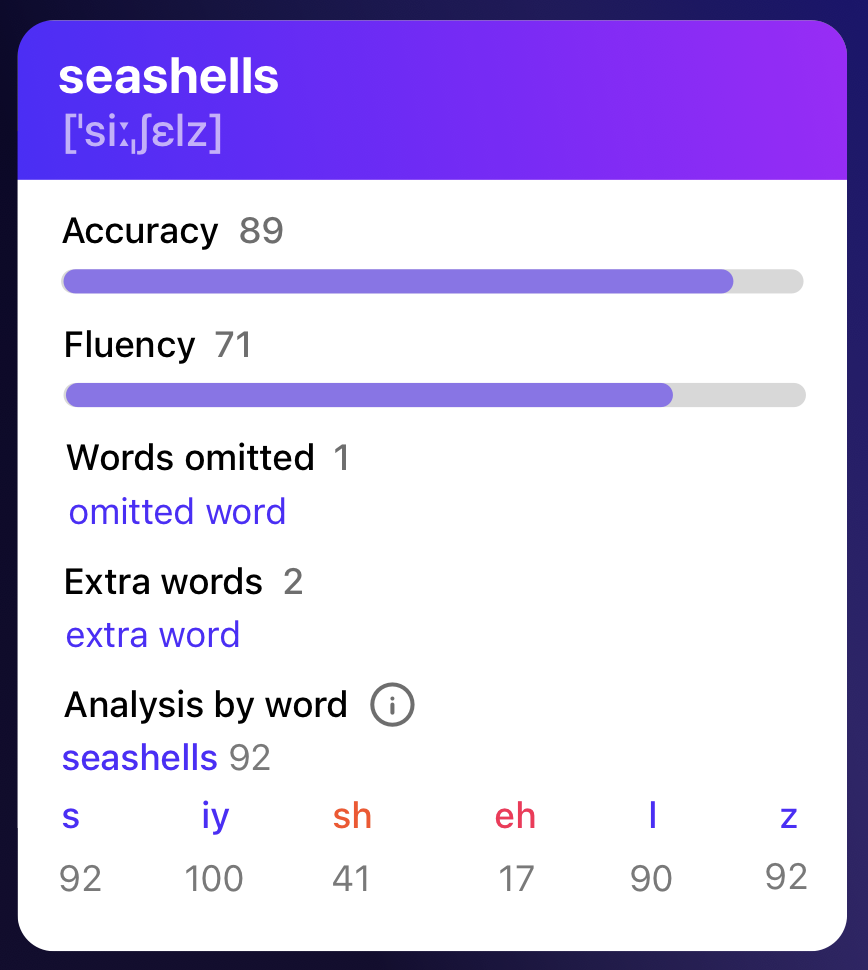
\includegraphics[width=0.5\textwidth]{pronunciation-card}
	\caption{Пример результата анализа произношения.}
	\label{fig:pronunciation-card}
\end{figure}

\subsubsection{Синтез речи}
Инструменты синтеза речи необходимы на этапе формирования изначальной базы слов, которая хранится в коллекции words. В качестве реализации механизма синтеза речи мы будем использовать один из инструментов Azure Cognitive Services, позволяющий генерировать качественную речь заданного содержания. На листинге \ref{lst:azure-pronunciation} приводится пример синтеза речи по фрагменту текста с последующим сохранением в файл.

\begin{lstlisting}[basicstyle=\fontsize{11}{11}\selectfont,tabsize=4,breaklines=true,caption={Пример проверки произношения с помощью Azure.},captionpos=b,label={lst:azure-pronunciation}]
const speechConfig = sdk.SpeechConfig.fromSubscription("key", "region");
const audioConfig = AudioConfig.fromAudioFileOutput("speech.wav");

const synthesizer = new SpeechSynthesizer(speechConfig, audioConfig);
synthesizer.speakTextAsync(
    "There's a difference between following the path and knowing the path.",
    result => {
        synthesizer.close();
        if (result) {
            return fs.createReadStream("speech.wav");
        }
    },
    error => {
        console.log(error);
        synthesizer.close();
    });
\end{lstlisting}

Результирующие звуковые файлы мы будем сохранять в Firebase Cloud Storage для дальнейшего использования в приложении. Ссылки на данные аудиофайлы в Storage также хранятся в документах коллекции words. Пример выгрузки аудио файла в Cloud Storage приводится на листинге \ref{lst:firebase-storage-upload}.

\begin{lstlisting}[basicstyle=\fontsize{11}{11}\selectfont,tabsize=4,breaklines=true,caption={Пример выгрузки аудио в Cloud Storage.},captionpos=b,label={lst:firebase-storage-upload}]
const config = // ...;
firebase.initializeApp(config);

const storage = firebase.storage();

const speechRef = storage.child('speech.wav');

speechRef.putFile('/path/to/file.wav').then(() => console.log('Audio uploaded!'));
\end{lstlisting}

\subsubsection{Классификация текстов по темам и сложности}
Классификация слов по темам и сложности также необходима не стадии формирования базы слов для обеспечения персонализированного подхода к обучению. Для оценки сложности и выборки тем, к которым может относиться слово, мы будем использовать TwinWord API\cite{twinword-overview}. Пример получения сложности слова приводится в листинге \ref{lst:word-difficulty}.

\begin{lstlisting}[basicstyle=\fontsize{11}{11}\selectfont,tabsize=4,breaklines=true,caption={Пример получения сложности слова.},captionpos=b,label={lst:word-difficulty}]
const axios = require('axios');

axios.post('https://twinword-language-scoring.p.rapidapi.com/word/', {
  entry: 'perseverance'
}, { headers: /* auth... */ })
  .then(response => console.log(response.data));
  // { ten_degree: 7, value: 0.49925, /* ... */ }
\end{lstlisting}

При помощи аналогичного запроса на листинге \ref{lst:word-topic} мы получим список тем, к которым относится слово.

\begin{lstlisting}[basicstyle=\fontsize{11}{11}\selectfont,tabsize=4,breaklines=true,caption={Пример получения тем, к которым относится слово.},captionpos=b,label={lst:word-topic}]
const axios = require('axios');

axios.post('https://twinword-topic-tagging.p.rapidapi.com/generate/', {
  text: 'perseverance'
}, { headers: /* auth... */ })
  .then(response => console.log(response.data));
  // { topic: { art: 0.2, machine: 0.23, technology: 0.18, study: 0.3 } }
\end{lstlisting}

API возвращает набор тем их весов, мы же для того, чтобы объединить большое количество разных тем объединяем эти темы в группы и смотрим на суммарные очки каждой группы. Темы, которые не попали ни в одну из групп, мы относим к категории <<общих>> слов. Таким образом мы объединяем десятки узко специализированных тем в несколько интересующих нас более широких.

\subsubsection{Генерация текста на заданную тематику}
Для генерации базы примеров мы используем два источника --- примеры из Azure Cognitive Services и автоматическую генерацию текста по заданному слову. Генерация текста производится с помощью API сервиса Inferkit (листинг \ref{lst:inferkit-generator}).

\begin{lstlisting}[basicstyle=\fontsize{11}{11}\selectfont,tabsize=4,breaklines=true,caption={Пример генерации текста с помощью Inferkit.},captionpos=b,label={lst:inferkit-generator}]
const axios = require('axios');

axios.post('https://api.inferkit.com/v1/models/standard/generate', {
  prompt: {
    text: "Perseverance"
  },
  length: 100,
}, { headers: /* auth... */ })
  .then(response => /* handling the reponse */);
\end{lstlisting}

Перевод текста на родной для студента язык производится с помощью Azure Cognitive Services.

\subsection{Вывод по разделу}
В разделе были представлены ключевые компоненты backend части приложения по изучению иностранных языков на React Native. 

Мы рассмотрели несколько платформ облачных вычислений, в частности, Google Cloud с Firebase и Microsoft Azure. Firebase является основой функционирования серверной части приложения, и все запросы приложение выполняет именно к нему.

Мы представили основные пункты реализации аутентификации пользователей с помощью Firebase. Далее была реализована работа с хранилищем данных приложения в Firestore, выделены основные структурные особенности.

Наконец, мы рассмотрели применение API различных сервисов, реализующих алгоритмы машинного обучения: Azure Cognitive Services, TwinWord и Inferkit. Мы применяем Azure для решения задач связанных с распознаванием речи, а остальные сервисы --- при работе с текстом.

В данном разделе мы построили реализацию backend части сервиса, завершая таким образом разработку приложения.
